
\subsection{Task Setting}



To demonstrate the critical role of hierarchical memory in long-horizon tasks, we designed three distinct tabletop manipulation scenarios, as illustrated in~\autoref{fig:exp}. These tasks are specifically curated to evaluate diverse capabilities, including user interaction, preference memory, updating memory and planning with exploration.

\textbf{Object Search.} 
We design a Domestic Maintenance task to evaluate the robot's capability to integrate inspection, sorting, and preference recall. In this scenario, the robot must first inspect opaque boxes to deduce storage rules and organize scattered items accordingly. Crucially, during this process, the user introduces new toys into the boxes to test the robot's ability to dynamically update its memory. Finally, the robot faces a retrieval challenge, where it must synthesize memorized user preferences with the box contents identified during inspection to retrieve the correct object.
% \textit{Evaluation metrics.} We evaluate the robot's proficiency by monitoring whether it performs necessary inspections, correctly memorizes box contents, places items in the appropriate containers, updates the memory with the latest observation and successfully retrieves the target object. 

\textbf{Counting.} 
In this scenario, the robot is required to interpret a visual recipe on the table and plan its subsequent actions. The task proceeds in stages: the robot must first \textit{inspect} the recipe to extract the ingredient composition and prepare the materials based on the number of servings requested by the user. Following this, the user introduces a specific preference. To fulfill this customized demand, the robot must synthesize the new constraint with the previously memorized recipe to dispense the correct personalized ingredients.
% \textit{Evaluation metrics.} We assess the robot's performance based on three criteria: (1) whether the robot actively and correctly inspected the visual recipe; (2) the accuracy of the ingredient preparation relative to the recipe and requested servings; and (3) whether the robot succeed in satisfying the final customized user preference.

\textbf{Rearrangement.} 
In this playroom scenario, the robot performs a two-stage ``clear and restore'' operation. Initially, the robot collects all toys scattered on the table into a storage box for cleaning. After a temporal interval, the robot is tasked with restoring the items to the environment. Crucially, the user's specific placement preference is provided beforehand as prior knowledge. Therefore, to execute the restoration, the robot must recall this pre-established preference and synthesize it with its visual memory of the original spatial configuration to plan the final placement of each item.
% \textit{Evaluation metric.} We measure task success based on two criteria: (1) the completeness of the initial collection into the storage box; and (2) the accuracy of the final restoration, specifically whether items were placed in the correct location.

\textbf{Evaluation Setup}
We use a WidowX-250s arm with a parallel gripper and dual-camera visual input (third-person and wrist view). The Executor $\pi_e$ runs at 2\,Hz, predicting an action chunk $A_t$ of 10 actions (10\,Hz), of which 5 are executed open-loop. To monitor the subtask progress, the Sentry $\pi_s$ is queried after every 10 execution steps of $\pi_e$. The Sentry will trigger Planner $\pi_p$ if the current subtask is completed for slow thinking.
Each task’s evaluation metrics are detailed in \autoref{app:eval}.




\subsection{Main Experiment}

% no memory: 只有 subtask， 1帧 GPT-4o+VLA (去掉planner和monitor）
% no memory + monitor： 只有 subtask， 8帧给 monitor 1帧给GPT-4o （去掉planner的memory能力）
% memer: planner只输出subtask， 超过 距离 8 则filter关键帧； 看临近8帧
% ours
% human 
% \paragraph{Main experiment.}

To thoroughly validate the effectiveness of our \emph{hierarchical memory} and the \emph{monitor-based} trigger mechanism, we keep the low-level policy $\pi_{\text{l}}$ and the planner backbone constant, varying only the \textbf{memory context} and the \textbf{planning frequency}. The comparisons are designed as follows:

% \siyin{add a table to compare all the methods: sentry/frequency(fix-interval vs trigger), memory (no, keyframe context, database)}
% (Place after "The comparisons are designed as follows:" or right before the itemize.)

% \begin{itemize} [itemsep=0.1em, topsep=0.3em]
%     \item \textbf{Transient Memory:} 
%     A standard hierarchical VLA baseline where a memory-less planner is invoked at fixed intervals ($n_m$) and observes only the current frame $o_t$. This represents the current paradigm of hierarchical robot foundation models, such as Hi-robot~\cite{Shi2025HiRO}.
%     % We remove the monitor module and the memory database. The planner $\pi_{\text{high}}$ is invoked at a fixed frequency and receives only the current frame $o_t$. This serves as a reactive baseline similar to standard hierachy VLA setups without temporal aggregation.
    
%     \item \textbf{Transient Memory w/ Sentry:} 
%     This variant introduces our Sentry module to trigger the planner based on task progress. However, the planner remains memory-less, receiving only $o_t$ upon being triggered. It evaluates the benefit of the more stablized planning from the sentry's gating.
%     % We introduce the monitor, providing it with the most recent 8 frames to decide whether the current subtask has terminated. However, when the planner is triggered, it still receives only the latest frame $o_t$ to predict the next subtask. This baseline isolates the benefit of the \emph{monitor's timing} from the \emph{planner's memory}.
    
%     \item \textbf{Flat Memory:} 
%     The planner operates at a fixed frequency and receives the 8 most recent observations, assisted by a FIFO queue of historical keyframes it previously selected. This setting tests whether unstructured, flat memory is sufficient for long-horizon tasks. This setting is similar to MemER \cite{Sridhar2025MemERSU}.
%     % To compare our hierarchical structure against flat retrieval methods, we implement a baseline inspired by MemER. The planner operates at a fixed frequency (without a monitor) and receives a context consisting of the recent 8 frames plus a FIFO queue of keyframes from the history. This tests whether unstructured keyframe retention is sufficient for long-horizon consistency.
    
%     \item \textbf{HiMe w/o Sentry:} 
%     We utilize our complete planner's memory design but remove the sentry module. The planner is forced to query the VLM at a fixed frequency regardless of subtask progress. This ablation validates the sentry's role in reducing computational redundancy and aligning planning steps with the dyanmics of environments.
    
%     \item \textbf{HiMe (Ours):} 
%     The proposed framework, where the monitor dynamically triggers planning based on subtask progress, and the planner utilizes the full hierarchical memory to ensure global consistency.
    
%     \item \textbf{Human High-level:} 
%     A human oracle provides the correct subtask description at each step. This serves as an upper bound on task performance given the fixed capabilities of $\pi_{\text{l}}$.

% \end{itemize}

\textbf{Transient Memory:} 
    A standard hierarchical VLA baseline where a memory-less planner is invoked at fixed intervals ($n_m$) and observes only the current frame $o_t$. This represents the current paradigm of hierarchical robot foundation models, such as Hi-robot~\cite{Shi2025HiRO}.
    % We remove the monitor module and the memory database. The planner $\pi_{\text{high}}$ is invoked at a fixed frequency and receives only the current frame $o_t$. This serves as a reactive baseline similar to standard hierachy VLA setups without temporal aggregation.
    
\textbf{Transient Memory w/ Sentry:} 
    This variant introduces our Sentry module to trigger the planner based on task progress. However, the planner remains memory-less, receiving only $o_t$ upon being triggered. It evaluates the benefit of the more stablized planning from the sentry's gating.
    % We introduce the monitor, providing it with the most recent 8 frames to decide whether the current subtask has terminated. However, when the planner is triggered, it still receives only the latest frame $o_t$ to predict the next subtask. This baseline isolates the benefit of the \emph{monitor's timing} from the \emph{planner's memory}.
    
\textbf{Flat Memory:} 
    The planner operates at a fixed frequency and receives the 8 most recent observations, assisted by a FIFO queue of historical keyframes it previously selected. This setting tests whether unstructured, flat memory is sufficient for long-horizon tasks. This setting is similar to MemER \cite{Sridhar2025MemERSU}.
    % To compare our hierarchical structure against flat retrieval methods, we implement a baseline inspired by MemER. The planner operates at a fixed frequency (without a monitor) and receives a context consisting of the recent 8 frames plus a FIFO queue of keyframes from the history. This tests whether unstructured keyframe retention is sufficient for long-horizon consistency.
    
\textbf{HiMe w/o Sentry:} 
    We utilize our complete planner's memory design but remove the sentry module. The planner is forced to query the VLM at a fixed frequency regardless of subtask progress. This ablation validates the sentry's role in reducing computational redundancy and aligning planning steps with the dyanmics of environments.
    
\textbf{HiMe (Ours):} 
    The proposed framework, where the Sentry dynamically triggers planning based on subtask progress, and the planner utilizes the full hierarchical memory to ensure global consistency.
    
\textbf{Human High-level:} 
    A human oracle provides the correct subtask description at each step. This serves as an upper bound on task performance given the fixed capabilities of $\pi_{l}$.


%  ===== Experiment Setting's Table =====
\newcommand{\TabW}{\dimexpr\columnwidth-6\tabcolsep\relax}

\begin{table}[t]
    \centering
    \small
    \setlength{\tabcolsep}{2.5pt}
    \renewcommand{\arraystretch}{1.12}
    % TODO: Adjust column width after content finalization
    \caption{
    Comparison of hierarchical settings in the main experiment. }
    \label{tab:main_settings}

    \begin{tabular}{@{}
    p{0.475\TabW}
    p{0.175\TabW}
    p{0.35\TabW}
    @{}}
        \toprule
        \textbf{Hierarchy Setting} & \textbf{Trigger} & \textbf{Planner Memory} \\
        \midrule
        Transient Memory
            & Periodic
            & Current observation \\
        Transient Memory w/ Sentry
            & Sentry
            & Current observation \\
        Flat Memory
            & Periodic
            & Recents + FIFO \\
        HiMe w/o Sentry
            & Periodic
            & Recents + keyframes \\
        HiMe (Ours)
            & Sentry
            & Recents + keyframes \\
        Human High-level
            & Sentry
            & Human oracle \\
        \bottomrule
    \end{tabular}
    \vspace{-0.6em}
\end{table}

% To validate the effectiveness of our proposed \emph{hierarchical memory} design, we keep the same low-level policy $\pi_{\text{low}}$ and high-level policy backbone $\pi_{\text{high}}$ across all settings, and \emph{only} vary the memory structure of $\pi_{\text{high}}$ (i.e., what context it observes and how it is invoked). This isolates the contribution of hierarchical memory from other confounding factors. We compare against the following baselines. 
% \emph{No memory}: we remove the monitor module and provide $\pi_{\text{high}}$ only the current frame at each planning step, requiring it to predict the subtask to execute next. 
% \emph{No memory w/ monitor}: we provide the monitor with the most recent 8 frames to decide whether the current subtask has terminated; however, each time the planner calls $\pi_{\text{high}}$, it still receives only the latest frame and must predict the next subtask. 
% \emph{Short memory + monitor}: building on \emph{No memory}, each planner call provides $\pi_{\text{high}}$ with 8 frames uniformly sampled from the execution history of the current subtask, and asks it to predict the next subtask. 
% \emph{MemER} 
% \emph{Ours}: a complete hierarchical memory design, 
% \emph{planner memory} similar to MemER
% Finally, we design a keyframe filter

% \emph{Human high-level}: a human oracle provides the correct subtask at each step, which serves as an upper bound on task performance given the fixed $\pi_{\text{low}}$.

% 这个主实验应该就是用来说明层次化记忆的用处
% 1. no memory VS no memory+monitor --》用来说明monitor的控制很重要(monitor拆解subtask，调节 planner的控制频率和vla的动作频率）
% 2. no memory+monitor VS  ours --》用来说明long-term memory的重要
% 3. no memory VS MemER vs Ours --> memer通过关键帧的筛选解决了一部分问题，但如果大模型做planner也会出现 仍然存在xx （


% \subsection{Q1: How much does the Sentry mechanism contribute to the overall performance?}
\subsection{Analysis of Sentry Mechanism}
\label{sec:sentry}
We analyze the Sentry mechanism's contribution from two key dimensions: \textit{execution consistency} and \textit{observation quality}.

\textit{1) Consistency via Reduced Task Switching:}
Even in a Planner with transient memory setting, the Sentry significantly boosts performance. 
In \autoref{fig:main}, we observe a substantial improvement ($14\%$ vs. $26\%$) when comparing \textit{Transient Memory} with \textit{Transient Memory w/ Sentry}. Without the Sentry, the planner operates on a frame-by-frame style, and this high-frequency re-evaluation makes the robot hypersensitive to transient visual noise, leading to frequent, erratic switching between subtasks. The Sentry prevent the planner from intervening until the current subtask is completed, reducing unnecessary task switching and ensures that actions are executed coherently. It reveals that \textbf{the core value of the Sentry here is enforcing temporal consistency of Planner.}

% Comparing \textit{Transient Memory} with \textit{Transient Memory w/ Sentry} (\autoref{fig:main}), we observe a substantial improvement ($14\%$ vs. $26\%$).
% \textbf{The core value of the Sentry here is enforcing temporal consistency.}
% Without the Sentry, the planner operates on a frame-by-frame basis. This high-frequency re-evaluation makes the agent hypersensitive to transient visual noise, leading to frequent, erratic switching between subtasks. The Sentry acts as a temporal lock, preventing the planner from intervening until the current subtask is completed. This reduces unnecessary task switching and ensures that actions are executed coherently.

\textit{2) Quality via Uniform Sampling vs. Recent Frames:}
% \siyin{experiment results --> conclusion.}
% Beyond consistency, the Sentry improves the quality of information provided to the planner.
% While a standard planner only sees a narrow window of recent frames, the Sentry accumulates the entire history of the executed subtask and provides a uniformly sampled overview.
% This is crucial for verifying success. A planner looking only at the last few frames might miss the context of the action, whereas the Sentry's global view allows the planner to verify the entire progression of the subtask, further reducing hallucination and replanning.

% Beyond consistency, the Sentry module significantly improves the quality of information provided to the planner, a benefit directly reflected in the substantial performance gap between \textbf{ours-sentry} and ours (\textbf{HiMe}).
% While the ablation model is constrained to a narrow window of recent frames, the Sentry accumulates the entire history of the executed subtask to provide a uniformly sampled overview.
% This global perspective is crucial for verifying success; for instance, a planner relying solely on recent observations might miss the context of an action, whereas the Sentry enables the verification of the entire subtask progression.
% Consequently, this capability to validate long-term execution effectively reduces hallucination and replanning, driving the average task progress from 68\% in \textbf{ours-sentry} to 90\% in \textbf{HiMe}.
% The Sentry's ability to consolidate raw observations into high-quality working memory is a primary factor in the performance gap between the \textit{HiMe w/o Sentry} and \textit{HiMe}, with average task progress increasing from $68\%$ to $90\%$. While standard planners are constrained to a narrow window of recent frames, the Sentry accumulates the entire history of the active subtask to form a structured working memory. By providing a uniformly sampled overview rather than transient snapshots, it offers a global perspective crucial for success verification. For instance, while recent frames may miss the full context of a physical interaction (e.g., the complete trajectory of a push), this consolidated working memory allows the Planner to verify the entire progression, effectively reducing hallucinations and redundant replanning.

The Sentry's ability to consolidate observations into high-quality working memory largely explains the gap between \textit{HiMe w/o Sentry} and \textit{HiMe}, with average task progress rising from $68\%$ to $90\%$. Whereas standard planners rely on a narrow window of recent frames, Sentry aggregates the history of the active subtask into structured working memory. This provides a global perspective for success verification, and the consolidated memory allows the Planner to verify the entire progression, effectively reducing hallucinations and redundant replanning.

\begin{figure*}
    \centering
    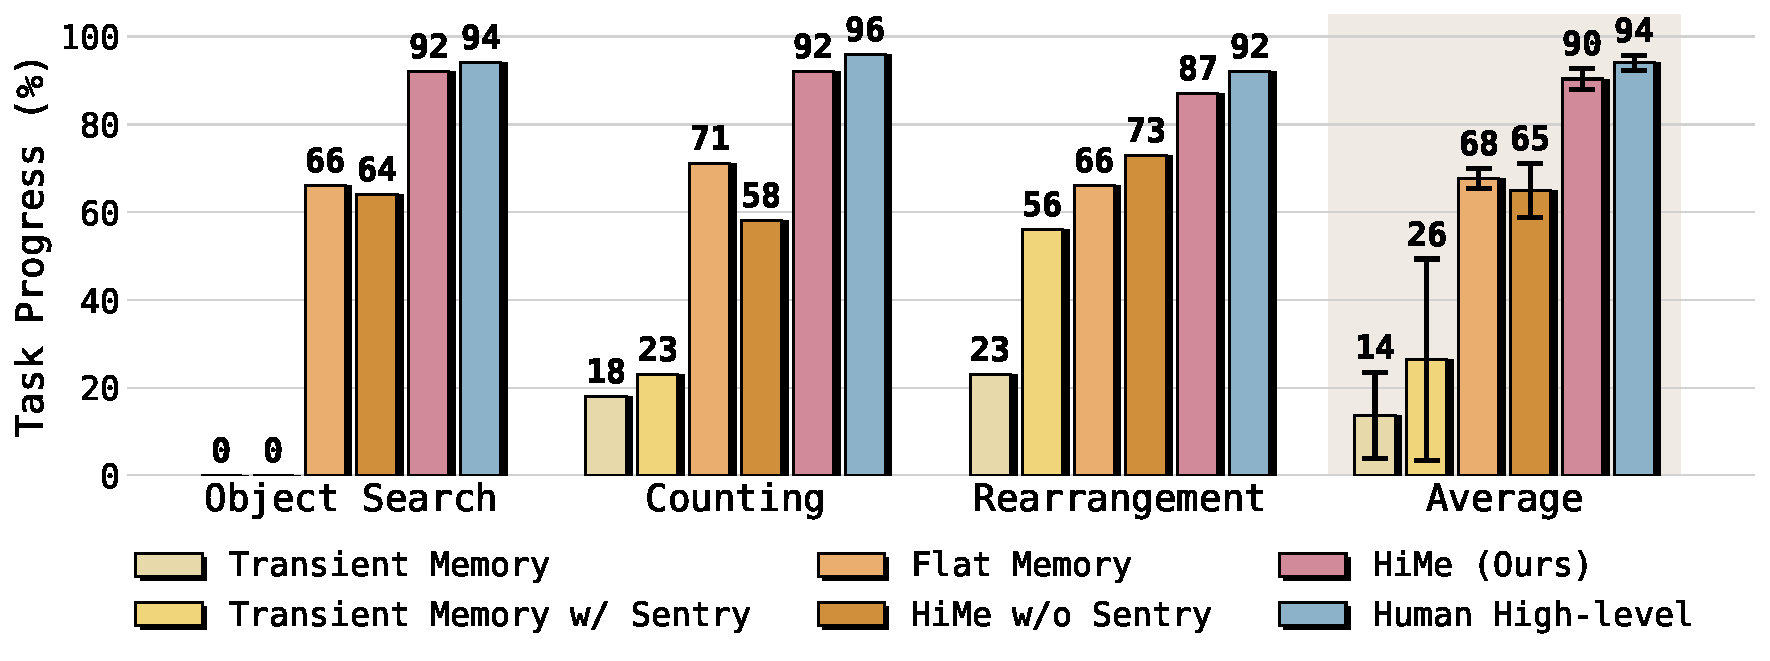
\includegraphics[width=0.98\linewidth]{imgs/6bars.pdf}
    \caption{\textbf{Main Results.} We compare HiMe against Transient, Sentry, and Flat Memory baselines across three long-horizon tasks. HiMe significantly outperforms all baselines, achieving a 90\% average success rate. Notably, our method effectively bridges the gap between robot and the Human High-level oracle.}
    \label{fig:main}
\end{figure*}


% \subsection{Q2: Effectiveness of Hierarchical Memory Architecture}
% \subsection{Q2: How does the Planner's episode memory management contribute to overall performance?}
\subsection{Analysis of Planner Memory Management}
\label{sec:memory}
We validate the necessity of our hierarchical design by comparing \textit{HiMe} against memory-free baselines and flat contextual memory approaches.

\textit{(1) The Necessity of Memory:}
% Long-horizon tasks impose strict requirements on state tracking. In the \textit{Counting} task, even with the Sentry's stability (\textit{No mem + sentry}), the agent fails ($23\%$) because it lacks persistence. Without an explicit memory module, the agent cannot retain states (e.g., counted objects) once they leave the immediate context window.
Long-horizon tasks require persistent state tracking. In \textit{Counting}, even with Sentry stabilization (\textit{Transient Memory w/ sentry}), the robot still fails ($23\%$) due to the lack of persistence: without an explicit memory management, it cannot retain states (e.g., counted objects) once they leave the transient observable state.

\textit{(2) Consolidation vs. FIFO Queues:}
A critical insight from \autoref{fig:main} is the inefficiency of \textit{Flat Memory}, which functions as a contextual memory based on FIFO queues. Although it stores history, it achieves a significantly lower task progress ($65\%$) compared to \textit{HiMe} ($90\%$).
The fundamental limitation of such contextual memory is the lack of consolidation: a simple FIFO queue cannot distinguish between truly critical frames and redundant observations.
In long-horizon tasks, the limited context window is quickly flooded with noisy frames, causing earlier critical information to be discarded. \textit{HiMe} addresses this by actively consolidating memory at the subtask level. This ensures that essential high-level information is preserved regardless of the episode length, enabling high-precision retrieval with minimal planner overhead. 



% \paragraph{Memory modality.}
% Robotic tasks impose heterogeneous memory requirements: the agent must retain \emph{visual} evidence (e.g., object locations and spatial relationships) while also tracking \emph{symbolic} and longitudinal information (e.g., user preferences, task progress, and constraints). Accordingly, we adopt a \textbf{hybrid image--text memory} as the default design, where each memory item can include both an image and a textual description. To assess whether multi-modal storage is necessary, we compare against two unimodal baselines. \emph{Image-only memory} restricts each entry to $(\text{tag}, \text{image}, \text{caption})$, where $\text{tag}$ and $\text{caption}$ are used only for indexing and retrieval, but the response to a query returns only the image. \emph{Text-only memory} restricts each entry to $(\text{tag}, \text{content})$ and enforces that $\text{content}$ is strictly textual (i.e., no images or visual representations).



\section{Further Analysis}

\subsection{Q1: What Type of Memory Representation is Most Effective for Robotic Tasks?}
We investigate the impact of memory modality by comparing purely text memory (\textit{Only text}), purely visual memory (\textit{Only image}), and our cross-modal approach. 

\textit{1) Spatial and Recognition Demands in Robotics:}
% Although many agentic memory systems opt for purely textual captions to minimize storage, our results suggest this is insufficient for physical interaction. Robotic tasks fundamentally rely on spatial relations, object localization, and precise recognition—information where visual data naturally excels.
% Relying solely on text becomes catastrophic when the initial perception model fails to fully recognize an object or accurately describe its spatial context. Text is a form of lossy compression; once the raw visual data is discarded, the robot loses the ability to perform visual re-grounding to recover these spatial details or correct initial recognition errors. In \textit{Object Search}, \textit{Only image} ($86\%$) significantly outperforms \textit{Only text} ($74\%$) for this reason.
Our study results show that robotics tasks impose strong spatial localization and fine-grained recognition demands that caption only memory is inadequate for dynamical physical interactions. Text is a lossy compression: if perception initially misses an object or its spatial context, discarding raw visuals prevents visual re-grounding to recover details or correct errors. In \textit{Object Search}, \textit{Only image} ($86\%$) substantially outperforms \textit{Only text} ($74\%$), which shows that memory with visual evidences is significantly stronger. 


\textit{2) Text for Semantics and Logic:}
% Conversely, text memory is indispensable for non-spatial reasoning. It is far more efficient for summarizing semantic information, analyzing logical dependencies (e.g., task sequencing), and retaining user preferences.
% In tasks requiring abstract reasoning like \textit{Counting}, \textit{Only text} ($91\%$) dominates \textit{Only image} ($78\%$), as these symbolic rules are difficult to extract from pixels on demand.
Conversely, text memory is indispensable for non-spatial reasoning. It efficiently summarizes semantics, captures logical dependencies like task sequencing, and retains user preferences. 
In tasks requiring semantic reasoning, such as \textit{Counting}, \textit{Only text} ($91\%$) outperforms \textit{Only image} ($78\%$), since these semantic clues are hard to extract from pixels on demand.


\textit{3) Superiority of Interleaved Memory:}
% Our cross-modal approach achieves the highest performance (Average $90\%$). By combining the spatial and recognitional fidelity of images with the semantic and logical structure of text, the system ensures the robot can both locate objects precisely in the physical world and reason effectively about user intent.
Our cross-modal approach achieves the best performance (Average $90\%$) by combining the spatial/recognitional fidelity of images with the semantic and logical structure of text, enabling our hierarchical memory system can perform both precise grounding and effective reasoning.



\begin{table*}[t]
\centering
% 使用 resizebox 确保表格适应页面宽度
\caption{Comparison of different methods. We report API calls, memory hit, and average scores across three tasks. Here, API Calls refers to the average Planner requests per subtask, and Memory Hit measures the presence of required information in memory during memory-dependent subtask.}\label{tab:comparison}
\resizebox{\textwidth}{!}{
\begin{tabular}{l ccc ccc ccc ccc}
\toprule
% 第一行表头：大标题
\textbf{Method} & \multicolumn{3}{c}{\textbf{Components}} & \multicolumn{3}{c}{\textbf{Search \& Retrieval}} & \multicolumn{3}{c}{\textbf{Counting}} & \multicolumn{3}{c}{\textbf{Clear \& Restore}} \\
\cmidrule(lr){2-4} \cmidrule(lr){5-7} \cmidrule(lr){8-10} \cmidrule(lr){11-13}

% 第二行表头：具体的列名
% Components 部分
 & \textbf{Sentry} 
 & \textbf{\begin{tabular}[b]{@{}c@{}}Memory\\Management\end{tabular}} 
 & \textbf{\begin{tabular}[b]{@{}c@{}}Memory\\Size\end{tabular}}
% Search & Retrieval 部分
 & \textbf{\begin{tabular}[b]{@{}c@{}}API\\Call ($\downarrow$)\end{tabular}} 
 & \textbf{\begin{tabular}[b]{@{}c@{}}Memory\\Hit ($\uparrow$)\end{tabular}} 
 & \textbf{\begin{tabular}[b]{@{}c@{}}Avg.\\Score ($\uparrow$)\end{tabular}} 
% Counting 部分
 & \textbf{\begin{tabular}[b]{@{}c@{}}API\\Call ($\downarrow$)\end{tabular}} 
 & \textbf{\begin{tabular}[b]{@{}c@{}}Memory\\Hit ($\uparrow$)\end{tabular}} 
 & \textbf{\begin{tabular}[b]{@{}c@{}}Avg.\\Score ($\uparrow$)\end{tabular}} 
% Clear & Restore 部分
 & \textbf{\begin{tabular}[b]{@{}c@{}}API\\Call ($\downarrow$)\end{tabular}} 
 & \textbf{\begin{tabular}[b]{@{}c@{}}Memory\\Hit ($\uparrow$)\end{tabular}} 
 & \textbf{\begin{tabular}[b]{@{}c@{}}Avg.\\Score ($\uparrow$)\end{tabular}} \\
\midrule

HiMe (Ours) & $\checkmark$ & $\checkmark$ & $infinite$ & \textbf{1.8} & \textbf{94\%} & \textbf{92\%} & \textbf{2.6} & \textbf{98\%} & \textbf{92\%} & \textbf{1.4} & \textbf{92\%} & \textbf{87\%} \\
Keyframe Memory & $\times$ & $\times$ & $recent \ 8$ & 5.4 & 68\% & 64\% & 4.8 & 61\% & 58\% & 6.2 & 76\% & 73\% \\
% HiMe w/o Sentry & $\checkmark$ & $\checkmark$ & $\times$ & 20 & 75\% & 0.82 & 15 & 70\% & 0.78 & 28 & 65\% & 0.72 \\
\bottomrule
\end{tabular}
}
\end{table*}
% \subsection{Q2: Are Dynamic Memory Maintenance (Update \& Delete) Necessary?}
\subsection{Q2: Are Dynamic Memory Management Necessary?}

% To validate the necessity of our proposed memory operations, we conducted an ablation study comparing our full method against two baselines: (1) \textit{No Management:} A baseline that only supports \texttt{Add} and \texttt{Retrieve} operations. It retains all historical observations without modification, effectively acting as an append-only buffer. (2) \textit{FIFO:} A variant of \textit{No Management} with a fixed memory capacity (8 entries). When the buffer is full, the earliest entries are evicted to make room for new ones.

To assess the need for dynamic memory management, we run an ablation against two baselines: (1) \textit{No Management}, which only supports \texttt{Add}/\texttt{Retrieve} and keeps all observations as an append-only buffer; and (2) \textit{FIFO}, which caps memory at 8 entries and evicts the oldest when full.

\textit{1) The Cost of Forgetting:}
% As shown in \autoref{fig:manage}, \textit{FIFO} performs the worst ($68\%$ average), significantly lagging behind \textit{No Management} ($86\%$). This performance drop demonstrates that in long-horizon tasks, \textbf{early historical context is crucial}. A fixed-size buffer with naive eviction discards essential information (e.g., the location of an object seen early in the episode) that is required for later reasoning.
In \autoref{fig:manage}, \textit{FIFO} performs worst ($68\%$ average), far below \textit{No Management} ($86\%$). This shows that for long-horizon tasks, \textbf{early context is critical}: naive eviction can remove essential information (e.g., an object location observed early) needed for later reasoning.

\textit{2) The Value of Consistency:}
While \textit{No Management} achieves decent performance by retaining all history, it is still inferior to our full method ($86\%$ vs. $90\%$).
% The limitation of \textit{No Management} lies in \textbf{redundancy and inconsistency}. Without the \textit{Update} and \textit{Delete} operations, the memory accumulates obsolete states (e.g., an object's previous location) alongside current states. This conflicting information introduces noise during the \textit{Query} process, potentially confusing the planner.
Although \textit{No Management} retains all history, it remains below our full method ($86\%$ vs. $90\%$) due to \textbf{redundancy and inconsistency}. Without \textit{Update}/\textit{Delete}, memory stores obsolete states (e.g., prior object locations) alongside current ones, introducing noise during \textit{Query} and potentially confusing the planner.

\textit{3) Necessity of Active Management:}
% Our method achieves the best performance by actively maintaining the memory. The \textit{Update} mechanism ensures state consistency by refreshing outdated entries, while \textit{Delete} removes redundancy. This proves that simply storing more data is not enough; the robot must actively curate its memory to maintain a concise and consistent memory.
Our method performs best by actively curating memory: \textit{Update} refreshes outdated entries to maintain consistency, and \textit{Delete} removes redundancy. Thus, storing more data is insufficient; effective robots must maintain a concise, consistent memory.



\begin{figure}
    \centering
    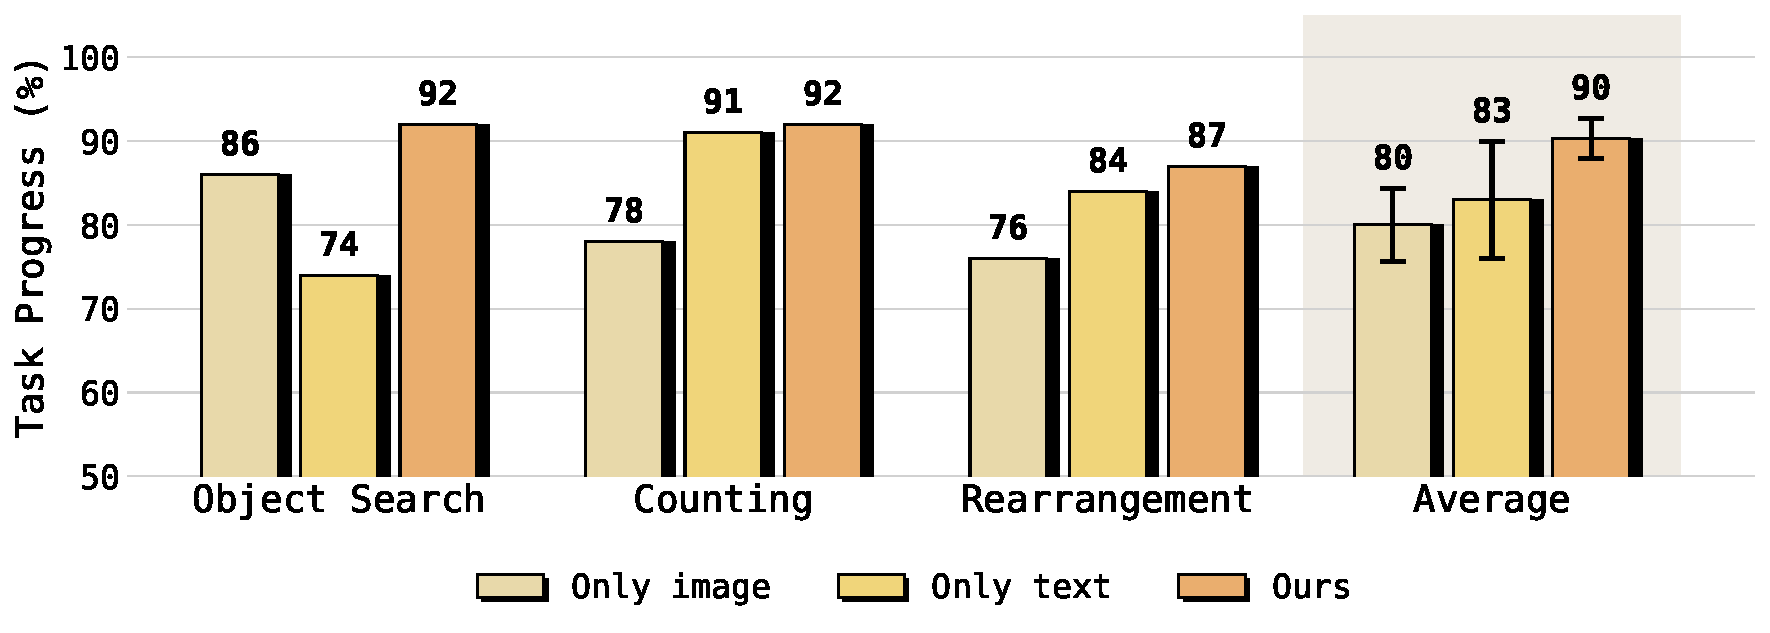
\includegraphics[width=1\linewidth]{imgs/modality.pdf}
    \caption{\textbf{Ablation of Modality.} HiMe consistently outperforms both text-only and image-only baselines across all three tasks, verifying the robustness of our cross-modal memory mechanism.}
    \label{fig:modality}
\end{figure}

% \paragraph{Memory management.}
% Beyond modality, we study whether explicit memory management improves robotic task performance. An effective memory system should remain accurate and up-to-date, reducing the impact of hallucination-induced erroneous entries and reflecting the current world state as the task progresses. We therefore compare our full method (supporting \emph{add/query/update/delete}) against two management baselines that only allow \emph{add} and \emph{query}: (i) \emph{No management}, which disables updates and deletions entirely while keeping all other settings fixed; and (ii) \emph{FIFO}, which maintains a fixed-capacity buffer of size $n$ (set to the average memory size observed under \emph{No management}) and evicts the oldest entries when full, mimicking a standard bounded replay buffer.


\begin{figure}
    \centering
    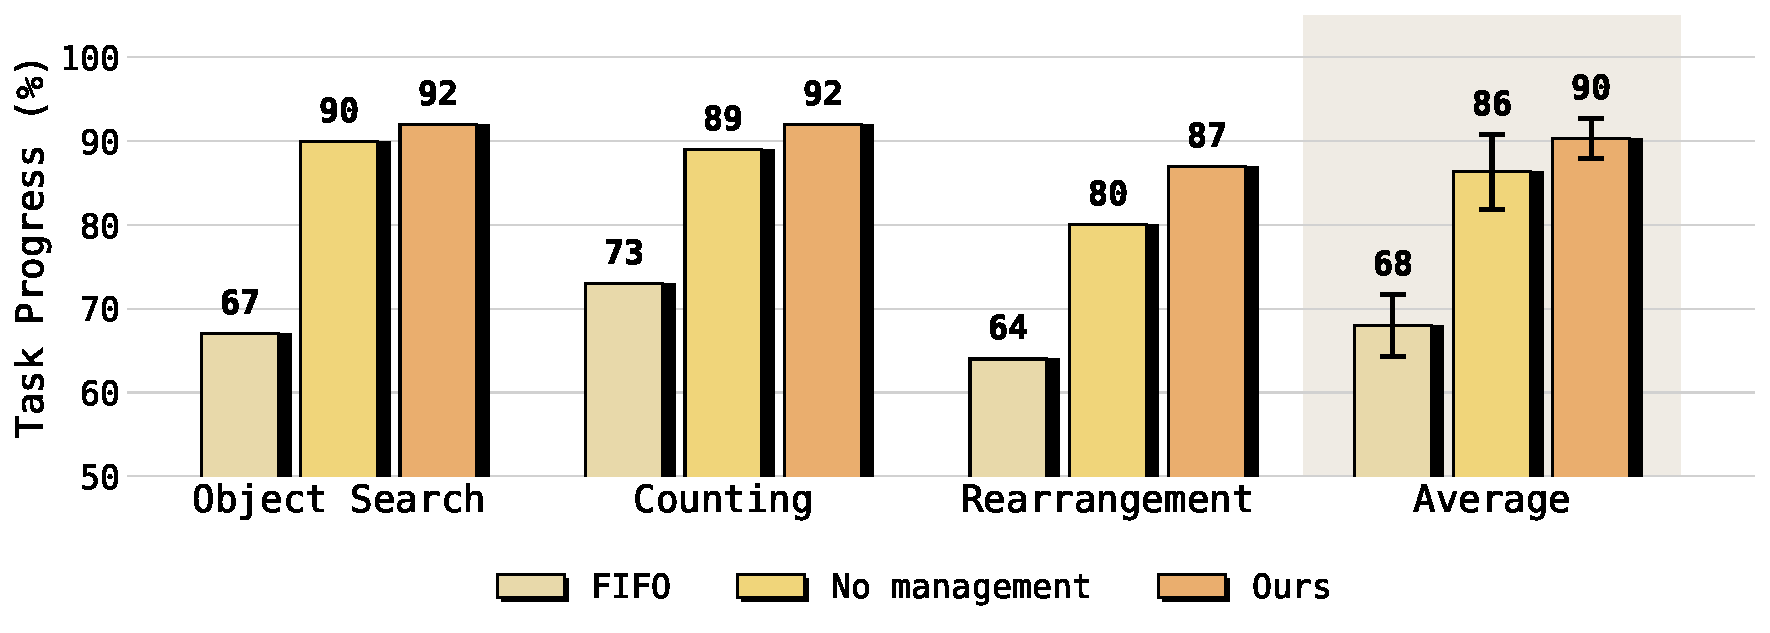
\includegraphics[width=1\linewidth]{imgs/management.pdf}
    \caption{\textbf{Ablation of Management.} Comparison between FIFO, No management, and our approach. HiMe consistently achieves the highest task progress across all three tasks, proving the effectiveness of our memory retrieval and consolidation mechanism in long-horizon tasks.}
    \label{fig:manage}
 \end{figure}

% \begin{figure}
%     \centering
%     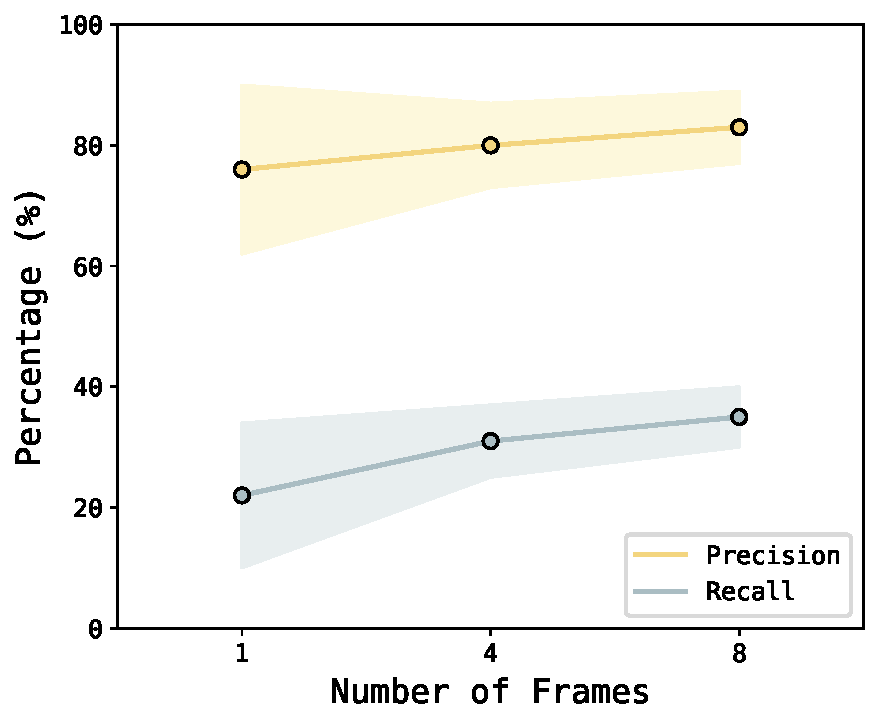
\includegraphics[width=1\linewidth]{imgs/window_sentry.pdf}
%     \caption{Increasing the number of recent frames provided to the Sentry leads to a consistent improvement in both precision and recall. This indicates that a longer temporal context is beneficial for accurate subtask monitoring.}
%     \label{fig:sentry_ablation}
% \end{figure}



\subsection{Q3: Why Does HiMe Achieve Lower Latency and Fewer API Calls?}
% We further analyze the efficiency and reliability of our method. 
% To quantify these metrics, we record the total Planner invocations during each test to determine the average \textit{API Calls} consumed per subtask. Simultaneously, we evaluate the \textit{Memory Hit} rate by verifying whether the requisite information is present in the memory whenever a subtask queries for historical context.
We further analyze efficiency and reliability by recording total Planner invocations (average \textit{API Calls} per subtask) and the \textit{Memory Hit} rate (whether required historical context is available at query time).

% While section~\autoref{sec:sentry} and \autoref{sec:memory} explain the performance gains, Table~\autoref{tab:comparison} reveals a significant efficiency advantage: HiMe reduces API calls by approximately $3\times$ (e.g., 5.4 to 1.8 in Search \& Retrieval) compared to the Flat memory. Since VLM inference is the dominant latency bottleneck, this reduction directly translates to faster execution. This efficiency stems from two structural advantages over the keyfra memory:
Beyond the gains in Sec.~\autoref{sec:sentry} and \autoref{sec:memory}, Table~\autoref{tab:comparison} shows a clear efficiency advantage: \textit{HiMe} reduces API calls by $\sim3\times$ (e.g., 5.4 to 1.8 in Search \& Retrieval) over Flat memory. Since VLM inference dominates latency, fewer calls directly yield faster execution. 
This efficiency stems from two structural advantages over the keyfra memory:

\textit{1) Sentry Reduces Invocation Frequency:}
% The primary driver for the reduction in API calls is the Sentry's role in the execution loop.
% In the Keyframe-based method, the Planner is typically queried at every step to interpret the visual buffer, placing the expensive LLM inside the high-frequency control loop.
% In contrast, our Sentry offloads the \textit{subtask completion check} from the Planner.
% Once the Planner defines a subtask (e.g., "inspect the recipe"), the Sentry takes over the dense verification loop, only waking the Planner upon completion or failure.
% This converts the Planner's involvement from a dense \textit{step-by-step} frequency to a sparse \textit{subtask-level} frequency.
In keyframe methods, the Planner is often queried every step to interpret the visual buffer, placing the expensive LLM in a high-frequency control loop. Our Sentry instead handles \textit{subtask completion checking} after the Planner specifies a subtask, it runs the dense verification loop and wakes the Planner only when necessary. Thus, Planner involvement shifts from \textit{step-by-step} to sparse \textit{subtask-level} calls.

\textit{2) Infinite Memory vs. FIFO Forgetting:}
% The second factor is the correlation between memory capacity and redundant actions.
% As shown in Table \autoref{tab:main_settings}, the \textit{Flat Memory} relies on a FIFO buffer of size 8. This creates a ``sliding window'' of context that inevitably forgets early observations as the episode progresses.
% The low memory hit rate ($68\%$ vs. $94\%$) reflects this limitation: when the Planner requires information about an object seen long time ago, the FIFO mechanism has already discarded it.
% Consequently, the agent is forced to issue redundant exploratory commands to re-acquire the lost context.
% By maintaining an infinite structured memory, HiMe prevents this catastrophic forgetting, allowing the agent to retrieve past observations instantly without physical re-exploration.
Flat Memory uses a FIFO buffer (\autoref{tab:main_settings}), forming a sliding window that forgets early observations. The resulting low memory hit rate ($68\%$ vs. $94\%$) forces redundant exploration when needed context has been evicted. In contrast, HiMe maintains an infinite structured memory, avoiding this forgetting and enabling immediate retrieval without physical re-exploration.

% 1. ours
% 2. only text
% 3. only image
% \subsection{Q6: Analysis of Sentry's Working Memory and Termination Policy}

% To understand the Sentry's decision-making boundary, we analyzed its performance on subtask completion detection under different working memory sizes (window length $N$). \autoref{fig:sentry_ablation} presents the Precision and Recall, where Subtask ``Done'' is treated as the positive class.

% \siyin{standardize the scale and all use percentages.}
% \textit{1) Benefits of Temporal Context:}
% As shown in the \autoref{fig:sentry_ablation}, increasing the context window from 1 to 8 frames improves both Precision (from $\sim76\%$ to $\sim82\%$) and Recall (from $\sim22\%$ to $\sim35\%$).
% A single frame often lacks sufficient information to distinguish between a temporary pause and true completion.
% By observing a sequence of 8 frames (consistent with our sentry‘s working memory), the Sentry can leverage temporal cues to make more reliable judgments.

% \textit{2) The "Conservative" Nature of Sentry:}
% The significant gap between high Precision and low Recall reveals the Sentry's inherent ``conservative'' nature.
% The system exhibits a strong bias towards the incomplete state, preferring to continue execution unless overwhelmingly confident that the goal is met.
% While this minimizes premature stops (high Precision), the low Recall creates a ``missing signal'' problem where the agent might overshoot its target or enter infinite loops.
% Since the Sentry is prone to False Negatives (missing the ``Done'' event), we design a fixed-interval Planner fallback.It ensures that execution loops are eventually broken even when the Sentry fails to trigger.




% \subsection{Q2: active management}
% 1. ours
% 2. only add
% 3. slide window

% monitor的working memory 有帮助 （定性/定量的设计
% 1. 8帧给monitor
% 2. 1帧给monitor
% 8B

% 成功的现象分析
% 错误分析 case study


% 【inference lantency？】
 

% 【subtask和plan要写进去吗？】

% 没有observer

% 记忆管理

% 记忆模态

% inference latency


% \subsection{failure taxonomy}


% 1. 普通的方法的常见问题往往出现在，错误的切换 subtask 导致 vla 进入 ood state； // 可以找一些 Planner Only 的方法中失效的案例，做定性对比分析。做配对的 frames 分析图（case-study）
% 7. 似乎ours - monitor 效果不好， 频繁决策下， plan list 是负面影响



% \paragraph{Over-replanning breeds instability: Reducing planning jitter improves execution stability. }

% Contrary to the intuition that higher reasoning frequency yields better performance, our empirical analysis reveals a 'Negative Influence' of excessive replanning. As illustrated in Fig. X, high-frequency updates to the Plan List introduce semantic chattering, where stochastic variations in VLM outputs force the Executor into frequent, unnecessary subtask switching. Our Sentry-governed hierarchy resolves this by enforcing temporal-logic commitment, allowing the robot to 'think slow' but 'act steady'.



% 视觉和文本记忆的重要性（需要记忆文本中的偏好 + 物体相似会出现混淆）

% 这个例子可以放在模态消融里搭配地讲
% 2. Off-the-shelf 的 vlm 随着时间的推移， 容易对任务中的物体发生混淆， 辨别失误；// ours: 我们的方法会存储图像缓解了模型混淆的情况
% 【不考虑】3. 单一的 memroy modality 方式的容错率低， (文本）容易受幻觉影响；【放在




% 【不写】6. 尽管是非记忆的任务， 但是当加入了memory ，例如 memer 或者 recent frame， 任务的效果也变好了， 有助于 model 去更好的认识自己的当前 state （working memory的重要

% Temporal context as a regularizer for state estimation.


% 5. 有时候对于记忆做出正确的利用了，但是没有保留下来 —— 没有 consolidation（放到论证为什么需要 memory database）
% "From Transient Context to Persistent Memory: Consolidation prevents the 'sliding window' forgetting.




% 4. Vlm 对于输入的图像的时序信息不敏感， 容易产生幻觉，将历史信息当作是当前 state；（暂时保留不写）



% 【不考虑】8. reset 的出现对于模型的 mdp 决策要求更高， 没有 plan list 有点难做
% 【不写】9. vlm 对于位置敏感， 对于物体名称不敏感 -- 对位置也不是很敏感， 分不清具体是哪个箱子;